\documentclass[10pt]{article}

\usepackage{float}
\usepackage[T1]{fontenc}
\usepackage[utf8]{inputenc}
\usepackage[english]{babel}
\usepackage{amssymb,amsfonts,amsmath,amsthm}
\usepackage{graphicx}
\usepackage{lmodern}
\usepackage{mdframed}
\usepackage{hyperref}
\usepackage{cases}
\usepackage{framed}
\usepackage{pdfpages}
\usepackage{multicol}
\usepackage[margin=60pt]{geometry}
\usepackage{abstract}
\renewcommand{\abstractnamefont}{\normalfont\Large\bfseries}
\renewcommand{\abstracttextfont}{\normalfont\normalsize}

\usepackage{pgfplots}
%\usepgfplotslibrary{colormaps}
\pgfplotsset{every axis/.append style={line width=1pt}}

\newcommand{\ud}{{\mathrm{d}}}
\newcommand{\pr}{{\mathbb{P}}}
\newcommand{\nN}{{n_\textrm{H}}}
\newcommand{\nI}{{n_\textrm{I}}}
\newcommand{\Xnema}{\textit{X. nematophila} }
\newcommand{\Scarpo}{\textit{S. carpocapsae} }
\newcommand{\Xenonema}{\textit{Xenorhabdus nematophila} }
\newcommand{\Steincarpo}{\textit{Steinernema carpocapsae} }
\newcommand{\Xeno}{\textit{Xenorhabdus} }
\newcommand{\Stein}{\textit{Steinernema} }
\newcommand{\Photo}{\textit{Photorhabdus} }
\newcommand{\Hetero}{\textit{Heterorhabditis} }
\newcommand{\IBD}{IBD}
\newcommand{\qw}{Q_\mathrm{w}}
\newcommand{\qb}{Q_\mathrm{b}}
\newcommand{\psis}{\psi}
\newcommand{\psic}{\psi}

\author{Latrille Thibault\\
\small thibault.latrille@ens-lyon.fr\\[-0.8ex]}
\title{Phenotypic variation as a cooperative strategy in \Xeno and \Photo}
\begin{document}
\includepdf[pages={1}]{first_page.pdf}
\begin{abstract}
Bacteria of the genera \Xeno and \Photo both colonize and influence the behavior of nematodes, \Stein and \Hetero respectively.
The nematodes infect, colonize and ultimately kill off an insect host, with the help of the bacteria.
Thus the bacteria are symbiotic of two hosts, as mutualistic symbiotes they help the nematode to reproduce optimally, as pathogenic symbiotes they are virulent toward the insect.
Many studies focused on the symbiotic association between the bacteria and their respective hosts, but they scarcely focused on cooperation among bacteria.
We will show that the life cycle of the bacteria is favorable to bacterial cooperation, as the life cycle allows for high relatedness among bacteria.
We here specifically investigated a trait of these bacteria observed experimentally: phenotypic variation. 
Isogenic bacteria are found in two phenotypic states that exhibits dramatically different physiologies. 
Phenotypic variation is here regarded as an evolutionary strategy.
We provide equations relating phenotypic variation frequencies in bacteria to demographic and migration parameters of the bacteria and their hosts. 
Our framework can be largely adapted to study manifold aspects of inclusive fitness of bacteria in the tripartite system bacteria-nematode-insect.

\smallskip
\noindent \textbf{Keywords.} Inclusive fitness, relatedness, phenotypic variation, \textit{Xenorhabdus}, \textit{Photorhabdus}.
\end{abstract}
\begin{multicols}{2}
\section*{Introduction}
\begin{figure*}[hbt!]
	  \centering
       \includegraphics[width=0.8\textwidth]{Figures/life_cycle.png}\\
		\caption{ \textbf{ The bacteria life cycle.} \label{fig:life_cycle}
		The infective juvenile nematode containing bacteria (nematode–bacteria complex) enters a susceptible insect host through natural openings that include the mouth, anus and spiracles.
		After entering the insect blood system, the nematode releases the bacteria.
		The bacteria undergo an exponential growth until the population reaches approximately $10^9$ bacteria, the growth is followed by a plateau.
		Together, the nematode and bacteria overcome insect immunity and kill the insect.
		The insect cadaver is used as a nutrient source and is protected from opportunistic infection and scavenging by metabolites produced by bacteria.
		Within this environment, nematodes reproduce sexually and progeny develop through four juvenile stages.
		Some nematodes develop into infective juveniles after being recolonized by their respective bacteria.
		The pair then exits the depleted insect carcass in search of a new host.}
\end{figure*}
\begin{figure*}[hbt!]
	  \centering
	  \label{fig:fitness}
       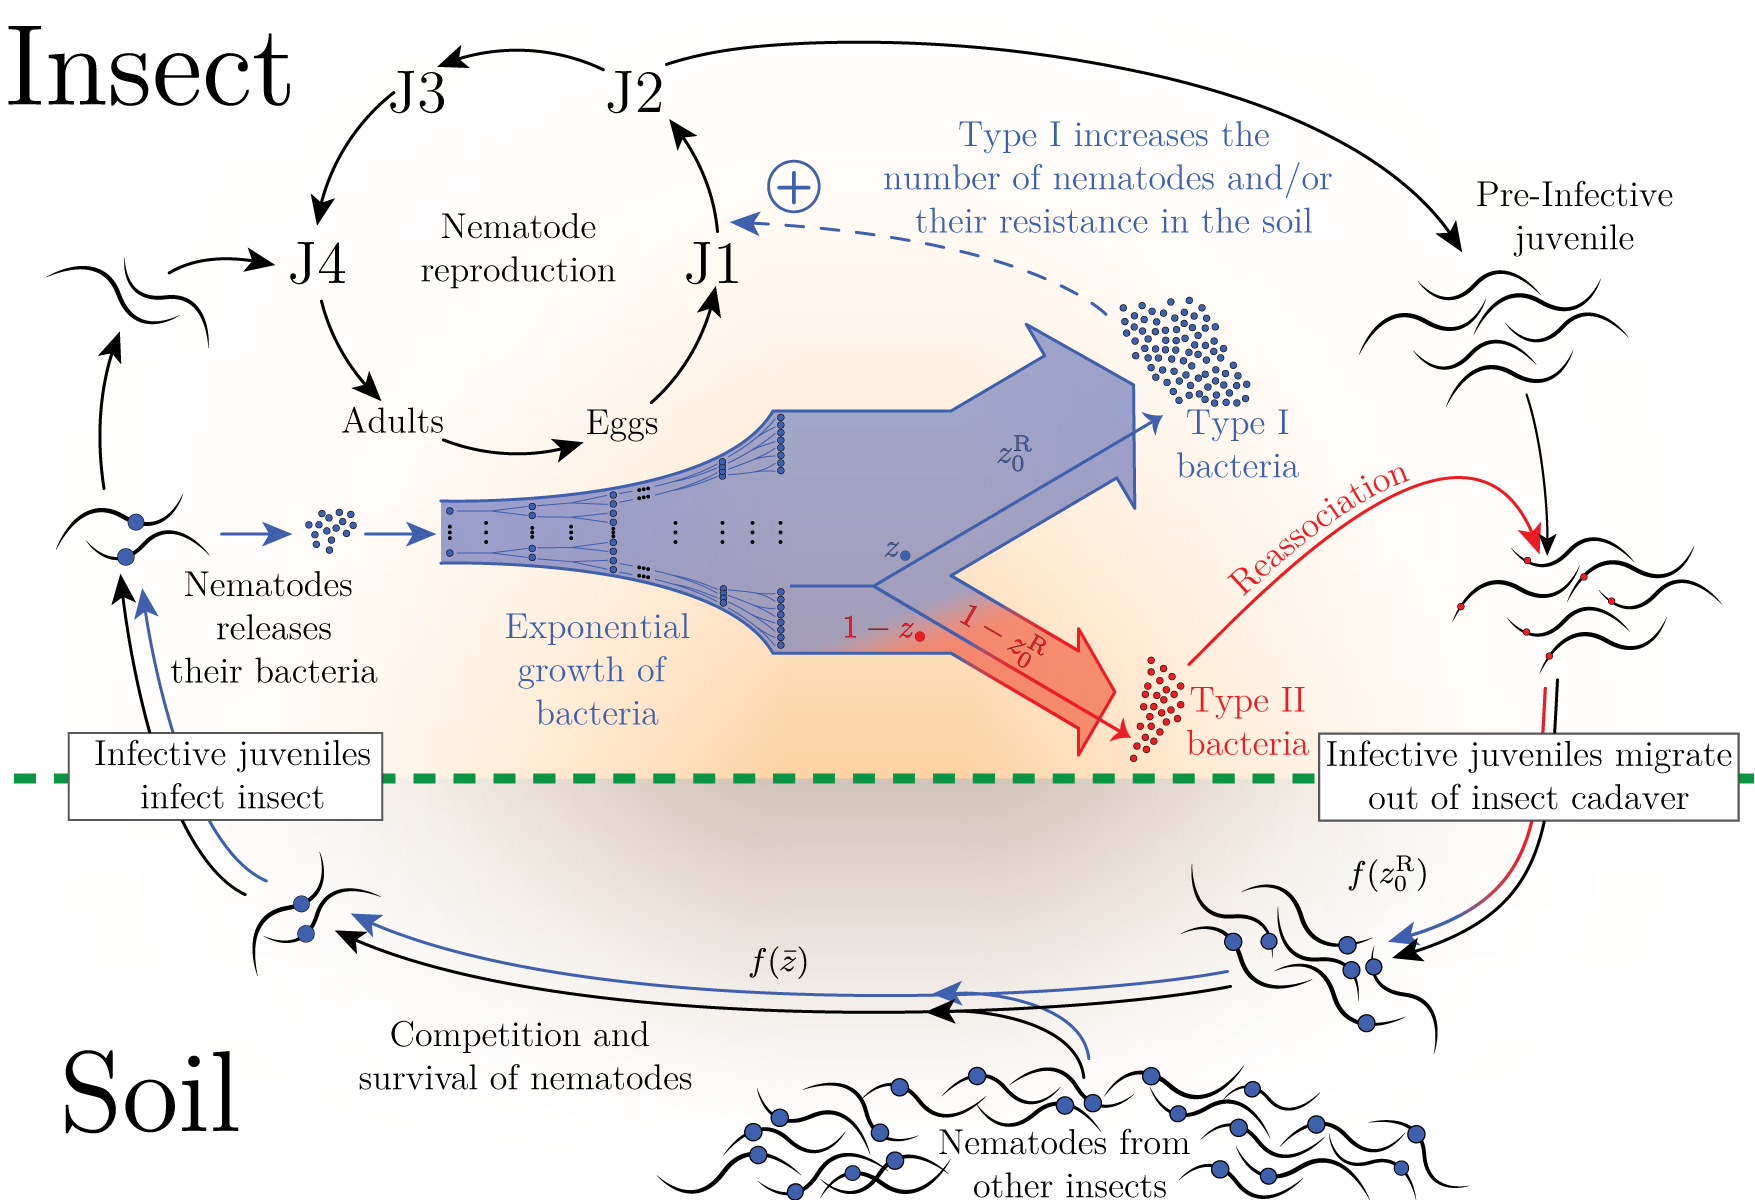
\includegraphics[width=0.8\textwidth]{Figures/fitness.png}\\
		\caption{\textbf{ The bacterial fitness along the life cycle.}
The life cycle is the same as in figure \ref{fig:life_cycle} but we introduce phenotypic variation, namely type I and II.
Type I are more virulent toward the insect, support nematode growth and development, eliminate unwanted guests but cannot associate with the nematode.
On the other hand, type II only associate to the nematode.
The phenotype under investigation, $z_\bullet$ is the probability that a focal lineage has not switched to type II by the time of colonization of a nematode by a bacterium.
$z_0^{\mathrm{R}}$ is the proportion of type I in the insect, and the survival of nematodes migrating out of the insect is $f(z_0^{\mathrm{R}})$.
The average success of nematodes migrating out of all insects is $f(\bar{z})$.
The fitness of a focal lineage is $(1-z_\bullet) f(z_0^{\mathrm{R}}) [(1- z_0^{\mathrm{R}})f(\bar{z})]^{-1}$.
We assume all bacteria switch back from type II to I during the soil dwelling stage.}
\end{figure*}
Studies of \Photo and \textit{Xenorhabdus} bacteria have significant potential to reveal both common and distinct aspects of pathogenesis and mutualism, as each of these bacteria naturally enter into both types of relationships during their life cycle: they are pathogens of insects and are mutualists of nematodes from the genus \Hetero and \Stein respectively \cite{Herbert2007,Akhurst1982a,Somvanshi2012}.
Most studies have been conducted on the species \Xenonema and \textit{Photorhabdus luminescens}, and their respective host \Steincarpo and \textit{Heterorhabditis bacteriophora}. For simplicity, we refer to these bacteria as \Xeno and \textit{Photorhabdus}.
%, although other species in these two genus may differ in various respects.

The mutualistic relationship between the bacteria and the nematode is not obligate, as both partners can survive in the absence of the other.
Thus, aposymbiotic \Stein nematodes can be obtained and assessed for responses to diverse bacterial and environmental stimuli.
However, symbiotic bacteria are required for nematodes to reproduce efficiently \cite{Sicard2003}.

Nematodes are either found in insect hosts or in the soil (Figure \ref{fig:life_cycle}).
The soil-dwelling vector stage, called the infective juvenile (IJ), is encased in a double cuticle, and is non-feeding owing to its closed mouth and anus.
Prior to the IJ stage, ingested bacteria colonize the nematode.
\Xeno colonize a discrete intestinal location known as the vesicle \cite{Chapuis2009}, which is the lumen between nematode epithelial cells at the anterior end of the intestine.
The \Xeno population within an IJ \Stein nematode is founded by one or two individual bacterial cells that grow to fill the vesicle.
The mature population contains between 50 and 100 colony-forming unit \cite{Martens}.
The specificity is stringent since other \Xeno species do not colonize \Scarpo IJs.
Conversely, \Photo bacteria occupy a substantial fraction of the lumen of the nematode gut\cite{Goodrich-Blair2007}.
The population is also founded by one or two individuals \cite{Somvanshi2012}.
Subsequently to colonization, the IJ nematode then serves as a vector, carrying bacteria into a susceptible insect, in which it is released from its nematode vector and rapidly kills the insect.
The bacteria are capable of killing insects in the absence of nematodes.

Haemolymph supports vigorous exponential growth \cite{Somvanshi2012} of bacteria, immediately upon release from the nematode.
By contrast, the nematode vesicle or gut is comparatively nutrient limiting.
The insect carcass thus provides nutrients for the propagation of both nematodes and bacteria.
In response to a signal, possibly nutrient deprivation or space limitation, bacteria re-associates with the nematode, and the pair leaves in search of a new insect host to repeat the cycle.
Nematodes are easily propagated; several hundred thousand IJs can be generated from the infection of a single insect host.

Although \Xnema and \Photo models are emerging as an invaluable tool for elucidating microorganism–host interactions,
many studies focused on the symbiotic association between the bacteria and their hosts, but they scarcely focused on interactions between bacteria.
We here seek to evaluate the potential for cooperation among bacteria.
We will show that the life cycle of the bacteria is favorable to bacterial cooperation.
To that aim we will formulate a condition for cooperation under simple scenarios consistent with knowledge of nematode-bacterial mutualism.
Our analysis uses well-established formalism to break down the condition for cooperation into the effect of different partners and their genetic relatedness.
We provide new results for relatedness, derived as a function of demographic parameters, experimentally accessible.
The relatedness in computed under a bacterial exponential stochastic growth process in the insect.
Although this framework can be adapted to study manifold aspects of inclusive fitness of bacteria, we have focused on a particular evolutionary strategy.
The bacteria can be found in two distinct phenotypic variant, whereas each variant exhibits dramatically different physiologies, required for initiating mutualistic or pathogenic life-styles \cite{Akhurst1982a,Forst1997}. 
In \textit{Photorhabdus0}, a stochastic promoter inversion causes the switch between the two variants \cite{Somvanshi2012}. The mecanism is yet unknown for \textit{Xenorhabdus}. 
We will formulate conditions for a candidate evolutionarily stable strategy \cite{lehmann2014fitness}, where the evolutionary strategy under investigation is the frequency at which the switch occurs.
This study is inspired by the tripartite symbiosis bacteria-nematode-insect, our aim is also to provide results more widely applicable.
The student derived the mathematical equations presented in this report, he also wrote C++ codes to validate the equations.
\section*{Phenotypic variation and inclusive fitness}

Both \Xeno and \Photo are found in the insect in two phenotypic variants \cite{Akhurst1982a,Forst1997}, denoted type I and II, controlled by a stochastic promoter inversion switch \cite{Somvanshi2012}.
Type I are known to be more virulent toward the insect than type II \cite{Volgyi,Givaudan2000}.
Type I are also known to produce crystal proteins \cite{Ciche2006,bintrim1998insertional} that supposedly nourish the nematode and support nematode growth and development \cite{Somvanshi2012}.
The nematodes also feed off and exploit the growing bacteria \cite{Waterfield2009}.
Furthermore, subsequently to the post-exponential phase of growth \cite{clarke1995virulence}, type I also produces bactericides \cite{Ji2004,Gualtieri2009} or fungicides that eliminate unwanted guests, thus increasing the foraging of the insect by the nematodes.
On the other hand, type II \Photo bacteria are known to better associate with the nematode, by producing proteins involved in recognition by the nematode \cite{Somvanshi2010,Heungens2002}.
Moreover, studies have shown that nematodes did not emerge from insect when infected by type II solely \cite{Sugar2012,Somvanshi2012}, suggesting the type I are required for nematode growth.

We hereby intend to model this phenomenon, using simplifying assumptions in order to produce analytic prediction. %\ref{fig:fitness}.
We assume that type I does not colonize any nematodes, but instead increase the number of nematodes that make it to the next cycle, or equivalently increase the survival of nematodes in the soil.
On the other hand type II are the ones that can colonize the nematodes.
This phenotype is only expressed after the exponential growth of bacteria, which holds experimental grounds \cite{Somvanshi2012}.
All bacteria switch back from type II to I during the soil dwelling stage of nematodes.

We seek to model the phenotypic variation as an evolutionary strategy acting upon fitness.
The phenotype under investigation is not expressed by a single bacteria, but instead should be seen as a phenotype expressed by a lineage of bacteria.
The resulting outcome on the bacteria at the end of the lineage is its type (I or II). $z$ is the probability that a lineage has not switched to type II by the time of colonization of a nematode by a bacterium.
The fitness of a focal lineage is a function of its own phenotype ($z_\bullet$), of the average phenotype of all lineages of bacteria in the same insect ($z_0^{\mathrm{R}}$), and the average phenotype of the total population over all insect hosts ($\bar{z}$).
By definition, $z_0^{\mathrm{R}}$ is thus the proportion of type I in the insect by the time of colonization of nematodes by bacteria, and $1-z_0^{\mathrm{R}}$ is the proportion of type II.
Similarly, $\bar{z}$ is the proportion of type I over all insects by the time of colonization of nematodes by bacteria, and $1-\bar{z}$ is the proportion of type II.

For a focal lineage, the probability that it ends colonizing a nematode is $1-z_\bullet$, and this lineage is competing with lineages that colonize nematodes with probability $1-z_0^{\mathrm{R}}$. Thus by solely taking into account colonization of the nematode, the fitness of a focal lineage is $(1- z_\bullet)/(1-z_0^{\mathrm{R}})$

However, the fitness of a focal lineage depends also on the survival of the nematodes migrating out the same insect.
While in turn, the survival of the nematode depends of the average phenotype of the lineages. 
We define a function $f$, which is the survival of nematodes as a function of the proportion of type I.
Upon colonization, the focal lineage is then carried over by nematodes from the same insect, thus with survival $f(z_0^{\mathrm{R}})$, competing with nematodes of average survival $f( \bar{z} )$. Thus by solely taking into account survival of the nematodes, the fitness of a focal lineage is $f(z_0^{\mathrm{R}})/f(\bar{z})$

  Taking into account the effect of both colonization and survival of the nematode, and under the model of infinite number of insects, the fitness $w(z_\bullet ,z_0^{\mathrm{R}} , \bar{z} )$ of a focal lineage is:
  \begin{equation}
  w(z_\bullet ,z_0^{\mathrm{R}} , \bar{z} ) = \dfrac{1- z_\bullet}{1-z_0^{\mathrm{R}}}\dfrac{f(z_0^{\mathrm{R}}) }{f(\bar{z})}
  \end{equation}
   We assume the success of nematodes $f$ is an increasing linear mapping of the proportion of type I: $f (x)=\alpha (x+\gamma)$, $\alpha>0$, $\gamma \geq 0$ thus leading to:
  \begin{equation}
  w(z_\bullet ,z_0^{\mathrm{R}} , \bar{z} ) = \dfrac{1- z_\bullet}{1-z_0^{\mathrm{R}}}\dfrac{ z_0^{\mathrm{R}} + \gamma }{ \bar{z} + \gamma}
  \end{equation}
  A framework to study evolutionary strategies is to look upon change in frequency of alleles over a life cycle \cite{Rousset2010Thegeneticaltheory,lehmann2014fitness}.
The change in frequency $\Delta p$ of a mutant allele (frequency $p$) with phenotype $z+\delta$ in a wild-type
population with phenotype $z$ is then given for a mutant with small phenotypic deviation $\delta$ by Lehmann \& Rousset (2014) \cite{lehmann2014fitness}:
  \begin{equation}
  \Delta p = p (1-p) \delta \left[ \left. \dfrac{\partial w}{\partial z_\bullet} \right\vert_{z^*} +  \dfrac{\mathrm{Cov}(z_\bullet,z_0^{\mathrm{R}})}{\mathrm{V}(\bar{z})} \left. \dfrac{\partial w}{\partial z_0^{\mathrm{R}}} \right\vert_{z^*} \right] + o ( \delta ).  \label{invasion}
  \end{equation}
  The regression coefficient $\dfrac{\mathrm{Cov}(z_\bullet,z_0^{\mathrm{R}})}{\mathrm{V}(\bar{z})}$ is also known as the relatedness ($R$), introduced initially by Hamilton \cite{Hamilton1964} and refined subsequently \cite{Lehmann2010a}. Statistically, the relatedness is the covariance between the mutant allele frequency in a focal individual and that in a recipient relative to the variance in mutant allele frequency in the population. 
The inclusive fitness thus take into account relatedness to break down change in frequency into the part due to the focal phenotype and the part due to phenotype of neighbors.

    A condition for a candidate evolutionarily stable strategy ($z^*$) is that no deviant mutant should invade the resident population. At equilibrium, the change of frequency of the mutant is null ($\Delta p=0$) and the equation \eqref{invasion} leads to:
    \begin{equation}
    \left. \dfrac{\partial w}{\partial z_\bullet} \right\vert_{z^*} +  R \left. \dfrac{\partial w}{\partial z_0^{\mathrm{R}}} \right\vert_{z^*} =0 \label{eqn:fit}\\
  \end{equation}
  We then need to compute the partial derivative of the fitness with respect to $z_\bullet$ and $z_0^{\mathrm{R}}$ and evaluate them at $z$:
  \begin{align}
   \left. \dfrac{\partial w(z_\bullet ,z_0^{\mathrm{R}} , \bar{z} )}{\partial z_\bullet} \right\vert_{z_\bullet = z_0^{\mathrm{R}} = \bar{z}=z} &= \dfrac{1}{ z-1 } \\
   \left. \dfrac{\partial w(z_\bullet ,z_0^{\mathrm{R}} , \bar{z} )}{\partial z_0^{\mathrm{R}}} \right\vert_{z_\bullet = z_0^{\mathrm{R}} = \bar{z}=z} &= \frac{1+\gamma}{(1-z)(z+\gamma )}.
  \end{align}
  Condition \eqref{eqn:fit} then implies:
    \begin{gather}
  \dfrac{1}{ z^*-1 } + R \frac{1+\gamma}{(1-z^*)(z^*+\gamma )} =0 \\
    \Rightarrow \nonumber \\
  z^*=R(1+ \gamma) - \gamma.
  \end{gather}
  In the special case $\gamma=0$ the phenotype is equal to the relatedness:
  \begin{equation}
  z^*=R.
  \end{equation}
  It is worth noting that if $R<\dfrac{\gamma}{\gamma+1}$, then the candidate evolutionarily stable strategy for a lineage is to switch necessarily to type II by the time of infection $(z^*=0)$.
  The next section is dedicated to derive the relatedness $R$ under various models of migration and infection.
\section*{Relatedness as a function of demographic and migration parameters}
\begin{figure*}[hbt!]
\begin{mdframed}
\begin{multicols}{2}
\textbf{Box 1: Proof of the equation \eqref{R_psi_phi_nI}\\}
\label{box:life_cycle_relatedness}
Let $Q_i$ be the probability of identity (PI) of genes from different bacteria. Within the same insect ($\qw$) and in different insect ($\qb$).
$\phi$ is the probability that two nematode infecting the same insect come from the same insect. $\phi$ is the correlation coefficient of migration. During the soil dwelling stage of nematodes and upon infection of the same insect, the PI within the same nematode is $Q_\mathrm{1}$ and the PI in different nematodes is $Q_\mathrm{2}$.
$\psi$ is the probability that two randomly chosen bacteria in the same insect originate from the same nematode, whenever nematodes arrive consecutively ($\psic$) or simultaneously ($\psis$).
We write the next generation identities $\qw '$ and $\qb '$ as.
\begin{subnumcases}{}
Q_\mathrm{1}=1 \label{sys:1}\\
Q_\mathrm{2}=\phi \qw +(1-\phi) \qb \label{sys:2} \\
\qw' = \psi Q_\mathrm{1} + (1- \psi) Q_\mathrm{2} \label{sys:3} \\
\qb' = \dfrac{ \qw }{\nI}+\dfrac{\nI-1}{\nI} \qb  \label{sys:4}
\end{subnumcases}
\begin{itemize}
	\item Upon infecting the same insect, bacteria in the same nematode \eqref{sys:1} are all clonal, originating from one bacterium that colonize the nematode.
	\item Upon infecting the same insect, bacteria in different nematodes \eqref{sys:2} come from the same insect with probability $\phi$ and thus have PI $\qw$, or come from different insect with probability $1-\phi$ and thus have PI $\qb $.
	\item In the same insect \eqref{sys:3}, bacteria come from the same nematodes with probability $ \psi $ and thus have PI $ Q_\mathrm{1} $, or come from different nematodes with probability $1- \psi $ and thus have PI $Q_\mathrm{2} $.
  \item In different insect \eqref{sys:4}, bacteria come from the same insect with probability $1/ \nI$ and thus have PI $\qw$,
  or come from different insects with probability $1- 1/ \nI$ and thus have PI $\qb$.
\end{itemize}
Putting together all the parts, in the infinite allele model with mutation rate $\mu$, the recursion equations for $\qw '$ and $\qb '$ are thus:
   \begin{subnumcases}{\hspace*{-1.cm}
   \label{sys2}}
      		 \qw ' = (1-\mu)^2[\psi + (1 -\psi) ( \phi \qw + (1-\phi) \qb ]  \\
    		 \qb ' = (1-\mu)^2 \left[ \dfrac{ \qw }{\nI}+\dfrac{\nI-1}{\nI} \qb \right].
  \end{subnumcases}
 \begin{figure}[H]
	\centering
  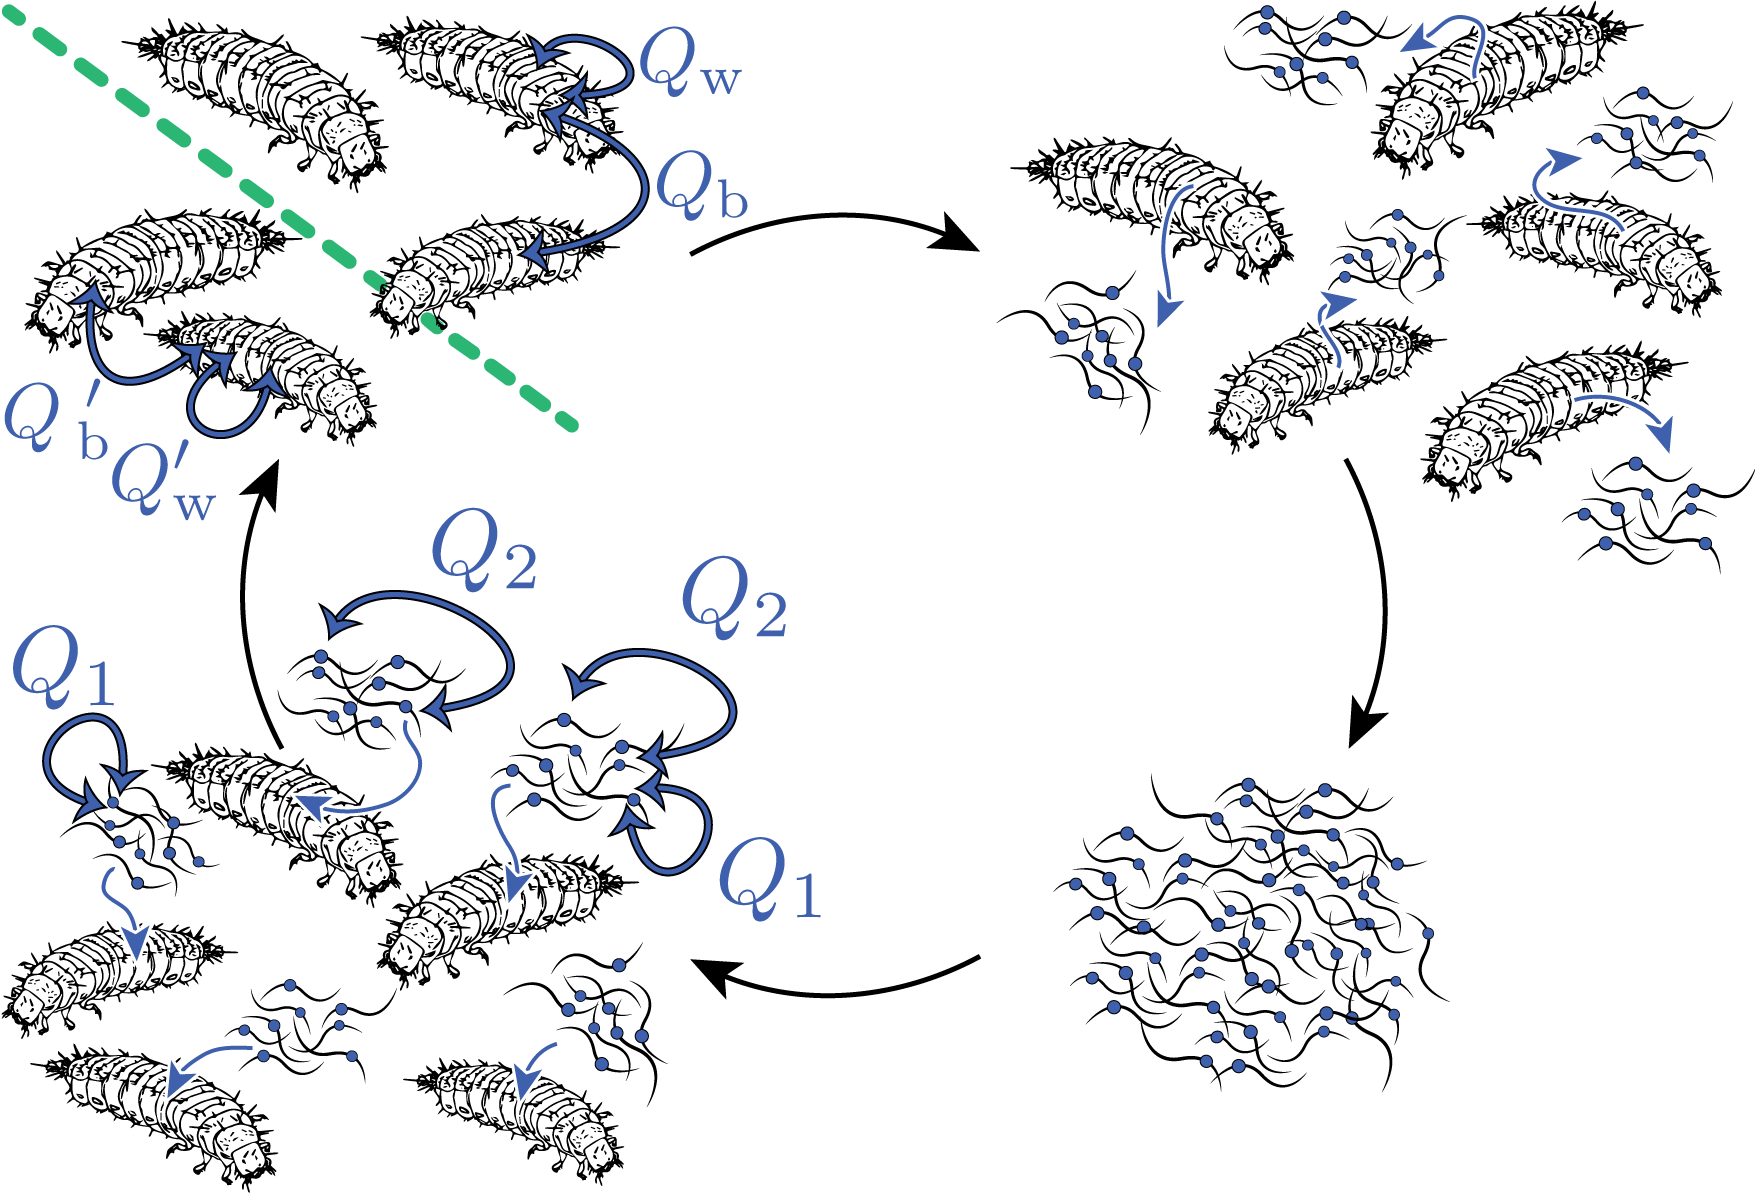
\includegraphics[width=\textwidth /2]{Figures/relatedness.png}\\
  \end{figure}
  At equilibrium, $\qw ' = \qw$ and $\qb ' =\qb$ and the recursion equations \eqref{sys2} can be solved explicitly and we have:
  \begin{equation}
\dfrac{\qw - \qb }{ 1- \qb } = \dfrac{ \psi (1-\mu)^2 }{ 1 - (1-\mu)^2 \phi (1- \psi )+(1-\mu)^2 / \nI } .
 \end{equation}
And thus by taking the limit for low mutation rate ($u \rightarrow 0$), the relatedness is \cite{rousset2004genetic}:
 \begin{align}
 R & = \lim_{\mu \rightarrow 0 }\dfrac{\qw - \qb }{ 1- \qb } \\
 &= \dfrac{ \psi  }{ 1 - \phi (1- \psi )+1 / \nI }.
 \end{align}
 \end{multicols}
 \end{mdframed}
\end{figure*}
\begin{figure*}[hbtp!]
\begin{mdframed}
\begin{multicols}{2}
\textbf{Box 2. Proof of the equation \eqref{eqn:star}}
\label{box:psi_simultaneous}
An insect is infected by $d$ nematodes.
Each nematode $i$ ($ 1 \leq i \ d$) releases his bacteria inside the insect.
The $d$ colonies of bacteria enter a stochastic growth process at time $t=0$.
In this context, $N_i(t)$ denotes the discrete random variable describing the population size of bacteria originating from the $i$th nematode, at time $t$.
$N_+(t)=\sum_{i=0}^d N_i(t)$ denotes the discrete random variable describing the size of the whole population of bacteria at time $t$.
The random variable $Z_i$ describes the frequency that two randomly chosen bacteria at time $t$ are originating from the $i$th nematode.
By definition we have:
\begin{equation}
Z_i=\dfrac{N_i(t)(N_i(t)-1)}{N_+(t)( N_+(t)-1 ) }.
\end{equation}
The expectation of the sum of $Z_i$ over all nematodes is thus $\psi (t)$, the probability
that two randomly chosen bacteria originate from the same nematode.
\begin{equation}
\psi(t) = \mathbb{E} \left[ \sum_{i=1}^d Z_i(t) \right] = \sum_{i=1}^d \mathbb{E}[ Z_i(t)]
\end{equation}
Thus we need to evaluate $\mathbb{E}[ Z_i(t)]$.
The growth process is modeled as a discrete space, continuous time Markov process. Each bacterium has an constant division rate $\lambda$ and they never die. Thus all bacteria is independent of one another. This model depicts an exponential growth.
$k_i$ denotes the number of bacteria initially contained in the $i$th nematode. The random variable $X_i(t)=N_i(t)-k_i$ is thus the number of births in the $i$th lineage. Under our model,
$X_i(t)$ is a negative binomial\cite[p. 158]{cox1977theory}:
\begin{equation}
X_i(t) \sim \mathrm{NB} \left( k_i, e^{-\lambda t} \right) \iff
\end{equation}
\begin{equation}
\pr(X_i(t)=x)=\binom{x+k_i -1}{x} \left( e^{-\lambda t} \right)^{k_i} \left( 1-e^{-\lambda t} \right)^{x}.
\end{equation}
Consistently with previous notations, $k_+=\sum_{i=0}^d k_i$ is the total number of bacteria released initially by the $d$ nematodes.
Equivalently $X_+(t)=N_+(t)-k_+$ is the total number of bacteria born. Since all $X_i(t)$ are independent of one another, $X_+(t)$ is also a negative binomial \cite{johnson2005univariate}:
\begin{equation}
 X_+(t)  \sim \mathrm{NB} \left( k_+, e^{-\lambda t} \right).
\end{equation}
Basic calculus leads to the distribution of $X_i(t)$ conditional on $ X_+(t)=x_+ $; this is a negative hypergeometric and independent of $e^{-\lambda t}$:
\begin{align}
\pr( X_i & (t) =x \vert X_+(t)=x_+ )  \nonumber \\
& = \dfrac{\displaystyle \binom{x+k_i-1}{x} \binom{x_+-x+k_+-k_i-1}{x_+-x}}{\displaystyle \binom{x_+ +k_+ -1}{x_+}}.
\end{align}
Leading to expectation for $X_i(t)(X_i(t)-1)$ conditional on $X_+(t)$:
\begin{align}
 \mathbb{E} [ X_i(t)& (X_i(t)-1) \vert X_+(t) ]  \nonumber \\
 &=\dfrac{k_i(k_i+1)}{k_+ (k_+ +1 )}X_+(t) ( X_+(t) -1 ).
\end{align}
And the expectation of $N_i(t)(N_i(t)-1)$ conditional on $N_+(t)$ is:
\begin{align}
 \mathbb{E} & [ N_i(t) (N_i(t)-1) \vert N_+(t) ]   \nonumber \\
 &=\dfrac{k_i(k_i+1) }{k_+ (k_+ +1)}N_+(t) ( N_+(t) -1 ) -\dfrac{2 k_i (k_+ - k_i) }{k_+ (k_+ +1)} N_+(t) .
\end{align}
Leading in turn to the expectation of $Z_i(t)$ conditional on $N_+(t)$.
\begin{align}
  \mathbb{E} [  Z_i(t)  & \vert N_+(t) ]  \nonumber \\
 &= \dfrac{k_i(k_i+1)}{k_+ (k_+ +1)}- \dfrac{2 k_i (k_+ -k_i)}{k_+ (k_+ +1)} \dfrac{1}{ N_+(t) -1  }.
\end{align}
By the law of conditional expectation:
\begin{align}
\mathbb{E}\left[ Z_i(t) \right] &=
 \mathbb{E}\left[ \mathbb{E}\left[ \left. Z_i(t) \right\vert N_+(t) \right] \right]\\
 &=\dfrac{k_i(k_i+1)}{k_+ (k_+ +1 )}-\dfrac{2 k_i (k_+ -k_i)}{k_+ (k_+ +1 )}\mathbb{E}\left[\dfrac{1}{N_+(t)-1} \right] \\
 & =\dfrac{k_i(k_i+1)}{k_+ (k_+ +1 )}-2e^{-\lambda t}\dfrac{ k_i (k_+ -k_i)}{k_+ (k_+^2 -1 )}.
\end{align}
By summing $\mathbb{E}\left[ Z_i(t) \right]$ over all $i$, we evaluate the probability of identity $\psi(t)$:
\begin{equation}
\psi(t) =\dfrac{ k_+ + \sum_{i=1}^d k_i^2}{k_+ (k_+ +1)}  -2 e^{-\lambda t} \dfrac{ k_+^2-\sum_{i=1}^d k_i^2}{k_+ (k_+^2 -1) }.
\end{equation}
Under the assumption that the number of bacteria carried by each nematode is large enough ($k_i \gg 1$), $\psi(t)$ becomes independent of $t$ and does not depend anymore on
 the bacteria growth rate:
 \begin{equation}
\psi \simeq \displaystyle \sum_{i=1}^d \left( \dfrac{ k_i}{\sum_{i=1}^d k_i} \right)^2.
 \end{equation}
 This approximation can be understood intuitively.
 If the initial number of bacteria if large enough, the probability that two randomly chosen bacteria originate from the same nematode is independent of time, and equals the sum over all nematodes of their squared initial proportions.
 \end{multicols}
 \end{mdframed}
\end{figure*}
 \begin{figure*}[hbt!]
\centering
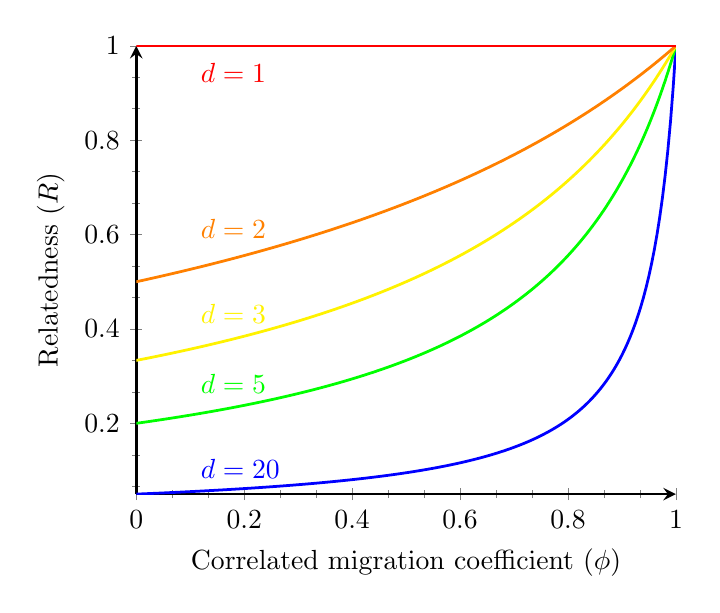
\begin{tikzpicture}
\begin{axis}[
ylabel={Relatedness ($R$)},
xlabel={Correlated migration coefficient ($\phi$)},
domain=0:1,
samples=201,
%legend entries={$d=20$,$d=5$,$d=3$, $d=2$,$d=1 $},
legend cell align=left,
minor tick num=2,
axis x line=bottom,
axis y line=left,
%legend style={at={(0.97,0.1)},anchor=south east}
]
\addplot[blue]{1 /(20 - (20-1)* x)};
\addplot[green]{1 /(5 - (5-1)* x)};
\addplot[yellow]{1 /(3 - (3-1)* x)};
\addplot[orange]{1 /(2 - (2-1)* x)};
\addplot[red]{1 /(1 - (1-1)* x)};
\node at (axis cs:0.1,0.06) [anchor=south west, blue] {$d=20$};
\node at (axis cs:0.1,0.24) [anchor=south west, green] {$d=5$};
\node at (axis cs:0.1,0.39) [anchor=south west, yellow] {$d=3$};
\node at (axis cs:0.1,0.57) [anchor=south west, orange] {$d=2$};
\node at (axis cs:0.1,0.9) [anchor=south west, red] {$d=1$};

\end{axis}
\end{tikzpicture}
\begin{tikzpicture}
\begin{axis}[
xlabel={Arrival rate relative to growth rate ($\omega$)},
ylabel={Relatedness ($R$)},
ymin=0.2, ymax=1,
legend cell align=left,
%minor tick num=2,
axis x line=bottom,
axis y line=left,
legend style={at={(1,0.95)},anchor=north east}
]
\addplot[green] table[x index=0,y index=2,col sep=space] {data/4nematodes_randtime_randgrowth.txt};
\addlegendentry{Average value for d=4}
\addplot[blue] table[x index=0,y index=2,col sep=space] {data/3nematodes_randtime_randgrowth.txt};
\addlegendentry{Average value for d=3}
\addplot[red] table[x index=0,y index=3 ,col sep=space] {data/2nematodes_randtime_randgrowth.txt};
\addlegendentry{95\% confidence bounds}
\addplot[black] table[x index=0,y index=1,col sep=space] {data/psic.dat};
\addlegendentry[black]{$1- 2 \omega \mathrm{B}_{1/2}(1+\omega,1-\omega)$}
\addplot[red] table[x index=0,y index=4,col sep=space] {data/2nematodes_randtime_randgrowth.txt};
\addplot[black, no markers, ultra thin] coordinates {(0,0.5) (5,0.5)};
\addplot[black, no markers, ultra thin] coordinates {(0,0.333) (5,0.333)};
\addplot[black, no markers, ultra thin] coordinates {(0,0.25) (5,0.25)};
\node at (axis cs:5,0.5+.02) [anchor=south east, red] {$d=2$};
\node at (axis cs:5,0.33+.02) [anchor=south east, blue] {$d=3$};
\node at (axis cs:5,0.25+.02) [anchor=south east, green] {$d=4$};
\end{axis}
\end{tikzpicture}
\caption{\textbf{Relatedness as a function of demographic parameters. Left panel:} Model of simultaneous infection.
Plot of the relatedness against $\phi$ \eqref{eqn:R_d_phi} for several values of $d$ ranging from $1$ to $20$. 
$\phi$ is the probability that two infecting nematodes come from the same insect.
$d$ is the number of nematodes infecting the insect.
If either the number of nematode is smalls or $\phi$ close to one, the relatedness is close to one. \textbf{Right panel:} 
The nematodes arrive consecutively, the time between two arrivals is $\mathrm{Exp}(\tau)$. The bacteria growth is exponential, with divisions at rate $\lambda$.
Estimated relatedness for $3$ and $4$ of nematodes (blue and purple solid lines) are plotted against the parameter $\omega=\tau \lambda^{-1}$.
For the case $d=2$, and under the assumption of a deterministic growth of bacteria, the relatedness is analytically derived (black solid line).
Red solid lines are the confidence bounds estimated from 1000 replicate simulations of growth within an insect.
If either the number of nematode is small or the arrival rate of nematodes is small or the growth rate of bacteria is large, the relatedness is close to one.\label{fig:R}}
\end{figure*}
\begin{figure*}[hbt!]
\begin{mdframed}
\begin{multicols}{2}
\textbf{Box 3. Proof of  the formula \eqref{eqn:star2}\\}
\label{box:psi_consecutive}
We derive an analytic formula for $\psic$ for two nematodes arriving successively.
We assume the first nematode arrive at time $T$ before the second (and last) nematode, where $T\sim \exp ( \tau)$.
Each nematode carries the same number of bacteria, $k \gg 1$.
The bacteria carried by the nematodes grew in a deterministic fashion at rate $\lambda$.
Under all these assumptions, the number of bacteria in the insect when the second nematode arrives is the random variable $k e^{\lambda  T}+k$.
Where $k e^{\lambda  T}$ bacteria are from the first one arrived and $k$ are from the second one.\\
  Since $k \gg 1$, the random variable $k e^{\lambda  T} $ is always far greater than $1$.
  Thus we can make use of the equation \eqref{eqn:star} to derive $\psic$:
  \begin{align}
  \psic  &=\mathbb{E} \left[ \left( \dfrac{ k e^{\lambda T}}{k+ke^{\lambda T}} \right)^2+\left( \dfrac{k}{k+ke^{\lambda T}} \right)^2 \right] \\
  &=\mathbb{E} \left[ \left( \dfrac{ e^{\lambda T}}{1+e^{\lambda T}} \right)^2+\left( \dfrac{1}{1+e^{\lambda T}} \right)^2 \right] \\
  &=\int_0^\infty \left( \left( \dfrac{ e^{\lambda t}}{1+e^{\lambda t}} \right)^2 + \left( \dfrac{1}{1+e^{\lambda t}} \right)^2 \right) \tau e^{ -\tau t } \ud t.
  \end{align}
  The evaluation of this integral is not straightforward.
  Instead we derive the cumulative distribution function $F_1(p)$ and $F_2(p)$ of $\dfrac{ e^{\lambda T}}{1+e^{\lambda T}}$ and $\dfrac{ 1}{1+e^{\lambda T}}$ respectively.
  \begin{align}
  F_1(p) &= \pr \left(\dfrac{e^{\lambda T}}{1+e^{\lambda T}} \leq p\right)= \pr \left(T \leq \lambda^{-1} \mathrm{ln}\left( \dfrac{p}{1-p} \right) \right) \nonumber \\
  &= 1-(1-p)^{\omega} p^{-\omega} \text{ for } 1/2 \leq p \leq 1,
  \end{align}
  where $\omega=\tau / \lambda$.
  \begin{align}
  F_2(p) &= \pr \left(\dfrac{1}{1+e^{\lambda T}} \leq p\right) = \pr \left(T \geq \lambda^{-1} \mathrm{ln}\left( \dfrac{1-p}{p} \right) \right) \nonumber \\
  &= (1-p)^{-\omega} p^\omega \text{ for } 0 \leq p \leq 1/2.
  \end{align}
  Hence the the probability density function $f_1(p)$ and $f_2(p)$ are:
  \begin{align}
  f_1(p) &= \dfrac{ \ud F_1(p) }{ \ud p} =  \omega (1-p)^{\omega-1} p^{-\omega-1}  \text{ for } 1/2 \leq p \leq 1,\\
  f_2(p) &= \dfrac{ \ud F_2(p) }{ \ud p} =  \omega (1-p)^{-\omega-1} p^{\omega-1} \text{ for } 0 \leq p \leq 1/2.
  \end{align}
  And
  \begin{align}
  \psic &= \int_{1/2}^{1} p^2 f_1(p) \ud p + \int_{0}^{1/2} p^2 f_2(p) \ud p \\
  &= 1 -2  \omega \int_{0}^{1/2}  (1-x)^{-\omega} x^{\omega}  \ud x \\
  &= 1- 2 \omega \mathrm{B}_{1/2}(1+\omega,1-\omega),
  \end{align}
  where $\mathrm{B}_x(a,b)$ is the incomplete beta function:
\begin{align}
\mathrm{B}_x(a,b) = \int_0^x t^{a-1}(1-t)^{b-1} \ud t.
\end{align}
  Thus the probability of identity is solely dependent on one parameter, $\omega$, the ratio between arrival rate of nematodes and growth rate of bacteria.
 \end{multicols}
\end{mdframed}
\end{figure*}
We seek to derive relatedness as a function of demographic and migration parameters.
The framework is largely inspired from Rousset \cite{rousset2004genetic}.
We developed two models.
In the first model, the insect is infected by nematodes arriving simultaneously. 
Moreover, the migration of nematodes is correlated, meaning the nematodes disperse in an aggregated pattern \cite{shapiro2013aggregative}.
% The group movement may have been continuous from the point of origin, or it may have been triggered by a propensity to aggregate after a short period of random movement.
In the second model, the insect is infected by nematodes arriving consecutively, but the migration is uncorrelated, meaning dispersal resulted in a random or uniform distribution.
\subsection*{Simultaneous infections, correlated migration}
The relatedness ($R$) is a regression coefficient, but $R$ can also be computed in terms of probability of identity \cite{rousset2004genetic}.
Let $Q_i$ be the probability of identity of genes from different bacteria, within the same insect ($\qw$) and in different insect ($\qb$).
Here we consider the probability of identity in the infinite allele model so that any mutation would lead to a different allele.
Let $\mu$ be the mutation rate.
The regression coefficient $R$ can be computed as \cite{rousset2004genetic}:
  \begin{equation}
 R = \lim_{\mu \rightarrow 0}\dfrac{\qw - \qb }{ 1- \qb }
 \end{equation}
 The $\qw$ and $\qb$ are obtained by solving recursions describing their change over successive life cycle, where parameters of these equations are relevant demographic and migration parameters (see Box \hyperref[box:life_cycle_relatedness]{1}).
 Thus the relatedness can be expressed as:
  \begin{equation}
 R \simeq \dfrac{ \psis  }{ 1 - \phi (1- \psis )+1 / \nI }.  \label{R_psi_phi_nI}
 \end{equation}
$\nI$ denotes the total number of insects.
$\phi$ is the probability that two infecting nematodes come from the same insect in the previous cycle.
The dispersal of nematodes is correlated, meaning nematodes preferentially follow other nematodes migrating out of the same insect.
 $\psis$ is the probability that two randomly chosen bacteria in the same insect originate from the same nematode.
Under the assumption of a large number of insects ($\nI \gg 1$), the relatedness $R$ is:
 \begin{equation}
 R  \simeq \dfrac{ \psis  }{ 1 - \phi (1- \psis ) }
 \end{equation}
Moreover $\psis$ can be derived explicitly (see Box \hyperref[box:psi_simultaneous]{2}) under assumption of a simultaneous infection by the nematodes.
The insect is infected by $d$ nematodes initially.
Each nematode $i$ ($ 1 \leq i \leq d$) releases $k_i$ bacteria inside the insect.
Then all $d$ lineages of bacteria enter a stochastic exponential growth process (at rate $\lambda$) simultaneously.
For a large number of bacteria carried by the nematode ($k_i \gg 1$), we have proved (see Box \hyperref[box:psi_simultaneous]{2}) that the stochastic part of the growth process is negligible. Thus $\psis$ is nearly independent of the time at which the growth is stopped in first approximation.
Moreover, $\psis$ is nearly independent of $\lambda$, and solely depends on the number of nematodes infecting the insect and their carrying capacities:
 \begin{equation}
\psis \simeq \displaystyle \sum_{i=1}^d \left( \dfrac{ k_i}{\sum_{i=1}^d k_i} \right)^2. \label{eqn:star}
 \end{equation}
If each nematode carries the same number of bacteria, $\psis$ reduces to:
\begin{equation}
\psis \simeq \dfrac{1}{d}
\end{equation}
The relatedness finally simplifies:
 \begin{align}
  R \simeq \dfrac{ 1  }{ d - \phi (d- 1 ) } \label{eqn:R_d_phi}
 \end{align}
 If either the number of nematodes infecting the insect ($d$) is small or $\phi$ close to one, the relatedness is close to one (see figure \ref{fig:R}).
\subsection*{Consecutive infections, uncorrelated migration}
The assumption of consecutive infections mainly affects the computation of $\psic$. The analysis of this scenario is otherwise similar to the previous one. R shall be given by equation \eqref{R_psi_phi_nI}.
 However, $\psic$ differs from the previous case. $\psic$ is the probability that two randomly chosen bacteria in the same insect originate from the same nematode, whenever nematodes arrive consecutively.
 In the case of uncorrelated migration, $\phi=1/ \nI$. Thus we have:
 \begin{equation}
 R \simeq \dfrac{\psic}{1+ \dfrac{\psic}{\nI}}.
 \end{equation}
Under the assumption of an important number of insects ($\nI \gg 1$), the relatedness is:
 \begin{equation}
 R \simeq \psic
 \end{equation}
 We seek to derive $\psic$ under assumption of a consecutive infections by the nematodes.
 The insect is infected by nematodes arriving successively.
We assume that the time elapsed between two nematode arrivals is exponentially distributed, with parameter $ \tau$.
$\tau$ is a rate measured per unit of time.
We assume a stochastic growth process for the bacteria, the division rate is $\lambda$, $\lambda$ is also measured per unit of time.
We could not derive an analytic formula of $\psic$ for this general case, instead we estimated it by simulating this process.
The results of these estimates are depicted in figure \ref{fig:R}. the C++ code is publicly available at \url{https://github.com/ThibaultLatrille/ISEM_M1_cpp_simulation}.
An analytical approximation in terms of the parameter $ \omega =\tau  \lambda^{-1}$ can be derived in the case $d=2$ (Box \hyperref[box:psi_consecutive]{3}), $\psis$ is a decreasing function of $ \omega $:
\begin{equation}
   \psic \simeq 1- 2 \omega \mathrm{B}_{1/2}(1+\omega,1-\omega) \label{eqn:star2},
\end{equation}
where $\mathrm{B}_x(a,b)$ is the incomplete beta function:
\begin{equation}
\mathrm{B}_x(a,b) = \int_0^x t^{a-1}(1-t)^{b-1} \ud t.
\end{equation}
This approximation, derived under the assumption that bacterial growth is deterministic matches well the simulation results (Figure \ref{fig:R}).

The relatedness increases with decreasing number of infecting nematodes, as in the previous model.
The relatedness also increases with decreasing arrival rate of nematodes or equivalently with increasing growth rate of bacteria.
Increasing growth rate or decreasing arrival rate leads to a population dominated by bacteria from the first nematode arrived.

The previous models could be combined to take into account both consecutive infections and correlated dispersal.
Nematodes move in aggregate, the aggregates arrive consecutively. The number of nematodes per aggregate is $d$.
In an aggregate, $\phi$ is the probability that two nematodes come from the same insect.
$\psis$ is the probability that two randomly chosen bacteria in the same insect originate from the same aggregate.
Thus $\psi$ shall be computed in terms of the number of aggregate, the time elapsed between two aggregate arrivals and the bacterial growth rate.
Using a similar framework as previously, we have:
\begin{equation}
   R = \dfrac{\psi}{d(1-\phi \psi)+\phi \psi}
\end{equation}
\section*{Discussion}
The parasitic life cycle of \Xeno and \Photo has an influence on their relatedness, and thus on the potential for cooperation among bacteria.
Under simplifying assumptions, we derive the candidate evolutionarily stable strategy for phenotypic variation probability switch.
This strategy is derived as a function of relatedness. The relatedness is subsequently derived as a function of a few demographic parameters, experimentally accessible.

Our model of simultaneous infection can be compared to outcomes of evolutionary experiments \cite{Vigneux2008}. Indeed, there is no experimental barrier to manipulate parameters such as $d$ or $\phi$ in the laboratory, thus the relatedness can be controlled and manipulated \cite{Vigneux2008}.
However, estimation of these parameters in the field seems complicated under this model of migration.
In the case of consecutive infection, if the division rate ($\lambda$) of bacteria can be hardly controlled but can be measured, the infection rate by nematodes ($\tau$) can be controlled in laboratory experiments.
The number of nematodes infecting the insects can also be controlled.
Moreover, estimating the arrival rate of nematodes is accessible in field experiments, assuming one can lure nematodes to a trap containing the insect and measure the arrival times.
Thus all demographic parameters can be estimated. 
Moreover, the relatedness can be estimated independently by various methods \cite{pamilo1982measuring}, and the results can be confronted to the prediction of demographic model to assess the validity of our model.

We focused on phenotypic variation since it holds experimental grounds, but experiments show contradictory results on many aspects \cite{Somvanshi2012}.
It is still unknown whether type I also colonize the nematode and to what extend which type contributes to the survival of nematodes \cite{Waterfield2009}. 
We investigated a plausible simple scenario in order to give insight on the relation between phenotypic traits and relatedness in both \Photo and \textit{Xenorhabdus}.
However, our model of phenotypic variation fits well with molecular and physiological data obtained on \textit{Photorhabdus} \cite{Somvanshi2012}, but the validity of this model need to further investigated for \Xeno bacteria. 

Our work is designed to encompass both \Photo and \Xeno similar life cycles.  
However, the molecular components of the regulatory networks controlling pathogenicity and mutualism in \Photo and \Xeno are different \cite{Goodrich-Blair2007}. 
Thus our prediction must be assessed on both models independently.

Our model can be incremented and adapted easily to take into account for known and future results.
The fitness function can be adapted to study other aspects of helping behaviors, not solely phenotypic variation.
By taking into account cooperation at the bacterial level, we hope this work will serve and drive new experiments on the tripartite system bacteria-nematode-insect.
\section*{Acknowledgments}
I thank François Rousset and Jean-Baptiste Ferdy for their help, support and advises all along the internship and concerning this report, as well as for insightful discussions.
I am grateful to my laptop who coped my relentless bashing.
\bibliographystyle{plain}
\bibliography{References_none_mendeley,References}
\end{multicols}
\end{document}
% \begin{tikzpicture}
%\begin{axis}[
%view={-45}{45},
%colorbar horizontal,
%colormap/temp,
%title={$R \simeq \dfrac{ \psi  }{ 1 - \phi (1- \psi )}$},
%xlabel={$\psi$},
%ylabel={$\phi$},
%]
%\addplot3[
%surf,
%domain=0:1,
%domain y=0:1,
%shader=faceted interp,
%draw=black,
%]
%{x /(1 - (1 - x)* y)};
%\end{axis}
%\end{tikzpicture}

